%*******10********20********30********40********50********60********70********80
\subsection{Uni-axial compression result for 10x10x10mm ASR Expanded Models}

In this section, simulation uni-axial compression test on a single aggregate case in size only 10x10x10mm is presented. Displacement of loading boundary is controlled in this analysis. In each step of loading, the top boundary of the concrete model moves downwards 0.002mm.

It is easier to analyze the behavior under loading condition in very small scale around coarse aggregate in a relatively smaller model.

The model is expanded by ASR following the process in chapter 2 and 3. 0.001 initial strain is introduced in each step at the interfaces between the aggregate and paste elements. Totally 20 steps of expansion are done.

%TODO: Single Aggregate 3D, 2D

\begin{figure}[h!]
\centering
%*******
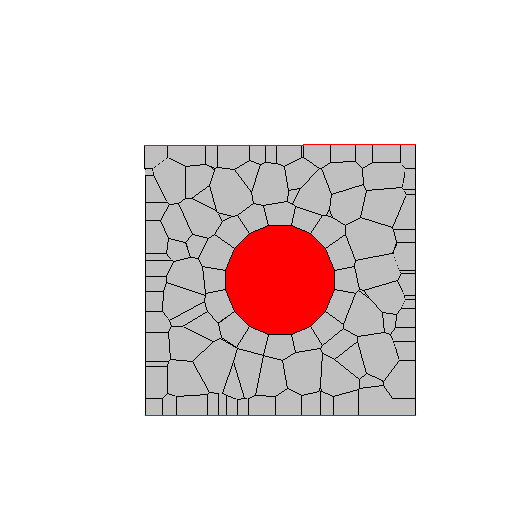
\includegraphics[width=0.4\linewidth]{Files/Small_ASR/CR/DEP5-STEP(001).png}
\caption{Single Aggregate Case in Size 10x10x10mm}
\end{figure}

\begin{figure}[ht!]
\centering

    %*******
    \begin{subfigure}{.33\textwidth}
      \centering
      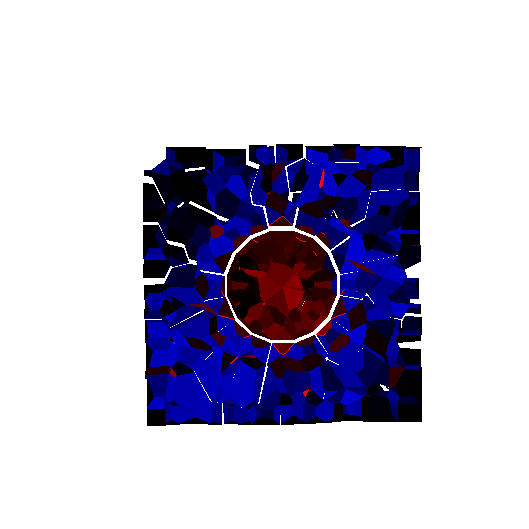
\includegraphics[width=1.0\linewidth]{Files/Small_ASR/IS2/DEP5-STEP(020).png}
      \caption{Before Loading}
    \end{subfigure}%
    \begin{subfigure}{.33\textwidth}
      \centering
      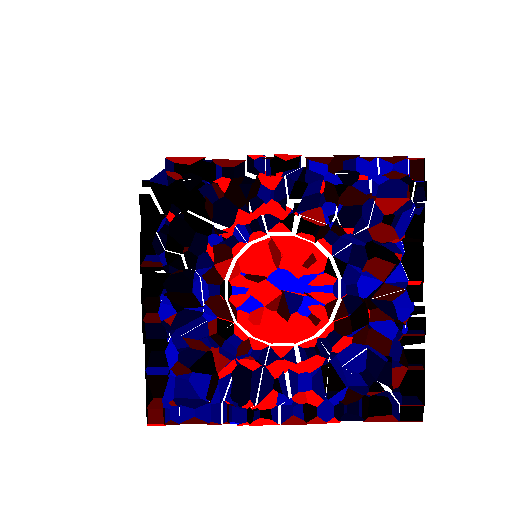
\includegraphics[width=1.0\linewidth]{Files/Small_ASR/IS2/DEP5-STEP(040).png}
      \caption{Loading Step 20}
      \end{subfigure}%
      %*******
      \begin{subfigure}{.33\textwidth}
        \centering
        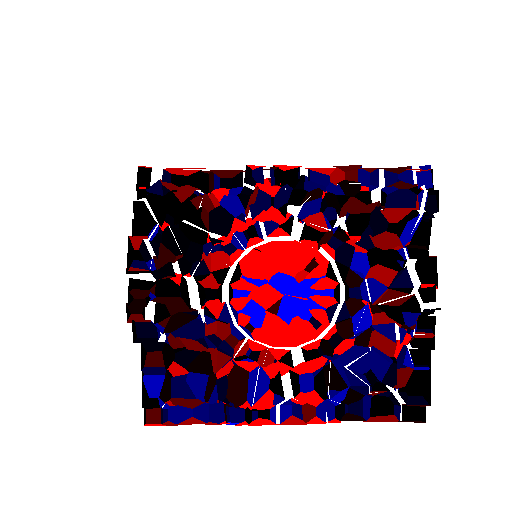
\includegraphics[width=1.0\linewidth]{Files/Small_ASR/IS2/DEP5-STEP(060).png}
        \caption{Loading Step 40}
      \end{subfigure}
      %*******

    %*******
    \begin{subfigure}{.33\textwidth}
      \centering
      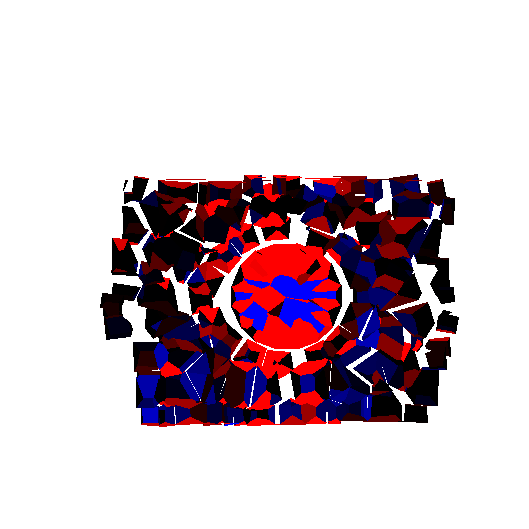
\includegraphics[width=1.0\linewidth]{Files/Small_ASR/IS2/DEP5-STEP(080).png}
      \caption{Loading Step 60}
    \end{subfigure}%
    \begin{subfigure}{.33\textwidth}
      \centering
      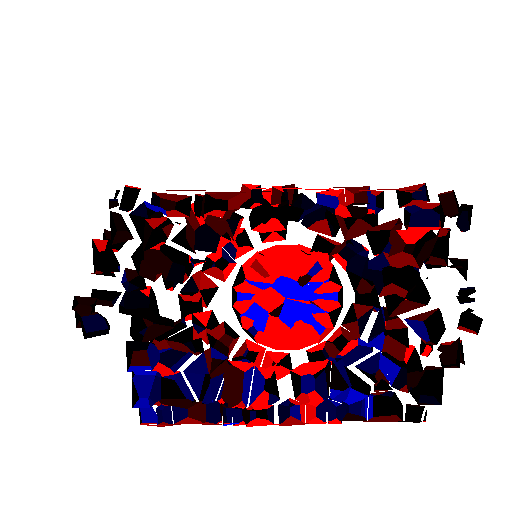
\includegraphics[width=1.0\linewidth]{Files/Small_ASR/IS2/DEP5-STEP(100).png}
      \caption{Loading Step 80}
      \end{subfigure}%
      %*******
      \begin{subfigure}{.33\textwidth}
        \centering
        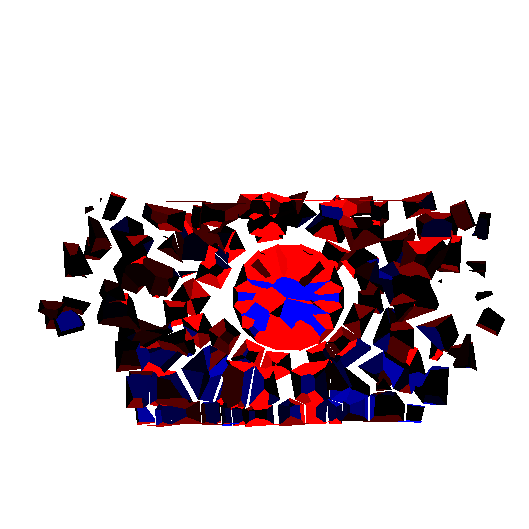
\includegraphics[width=1.0\linewidth]{Files/Small_ASR/IS2/DEP5-STEP(120).png}
        \caption{Loading Step 100}
      \end{subfigure}
      %*******

  \caption{ASR Loading for 10x10x10mm model, Fixed Boundary Condition}
  \label{fig:ASR_Loading_s_fix}
\end{figure}

For Loading with fixed boundary condition, Figure \ref{fig:ASR_Loading_s_fix} here shows the initial stress condition during loading in loading step 0, 20, 30, 60 and 80.

With increasing the step of loading, in each step the top surface moves downwards for 0.002mm. Compressive strength generate together with the deformation, especially concentrated horizontally in the middle of the model.

As the top and bottom boundary are horizontally, elements in the middle of model start to move away from the center of model firstly, followed by the failure of whole model.

If we compare its behavior with free boundary condition loading, shown in Figure \ref{fig:ASR_Loading_s_free}, it can be seen that the way crack generate and deformation generate is totally different in these two cases.

In Free boundary loading, the cracks are more easier to open without the restrain from top and bottom boundary. The deformation in horizontal direction is more uniformed. Inner Stress distributed more uniformly in the free boundary loading case.

\begin{figure}[ht!]
\centering

    %*******
    \begin{subfigure}{.33\textwidth}
      \centering
      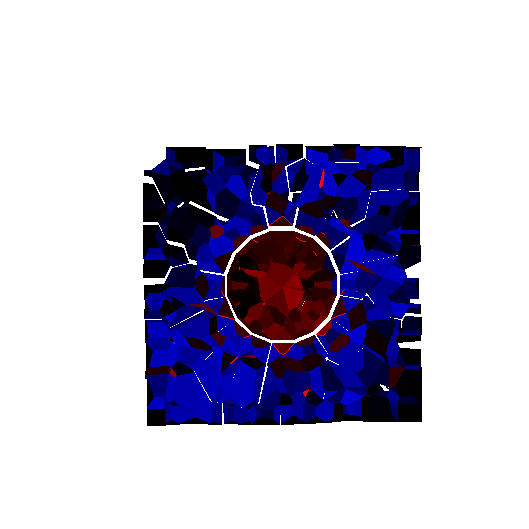
\includegraphics[width=1.0\linewidth]{Files/Small_ASR/IS2/DEP5-STEP(020).png}
      \caption{Before Loading}
    \end{subfigure}%
    \begin{subfigure}{.33\textwidth}
      \centering
      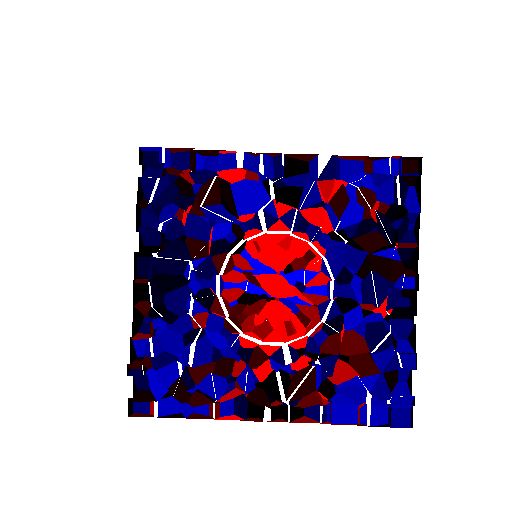
\includegraphics[width=1.0\linewidth]{Files/Small_ASR/Free_IS2/DEP5-STEP(040).png}
      \caption{Loading Step 20}
      \end{subfigure}%
      %*******
      \begin{subfigure}{.33\textwidth}
        \centering
        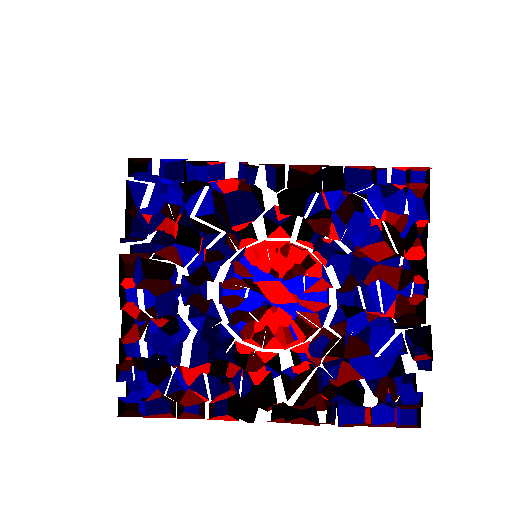
\includegraphics[width=1.0\linewidth]{Files/Small_ASR/Free_IS2/DEP5-STEP(060).png}
        \caption{Loading Step 40}
      \end{subfigure}
      %*******

    %*******
    \begin{subfigure}{.33\textwidth}
      \centering
      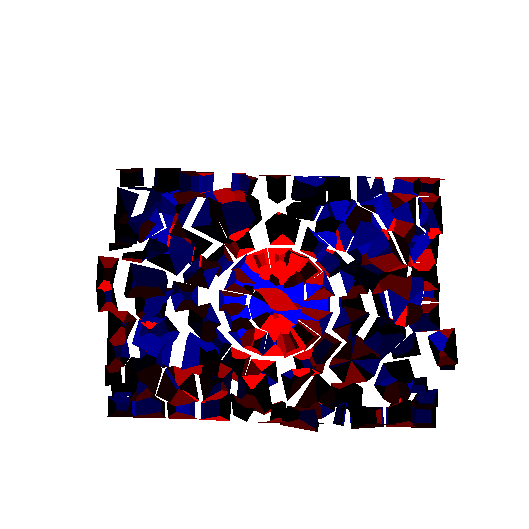
\includegraphics[width=1.0\linewidth]{Files/Small_ASR/Free_IS2/DEP5-STEP(080).png}
      \caption{Loading Step 60}
    \end{subfigure}%
    \begin{subfigure}{.33\textwidth}
      \centering
      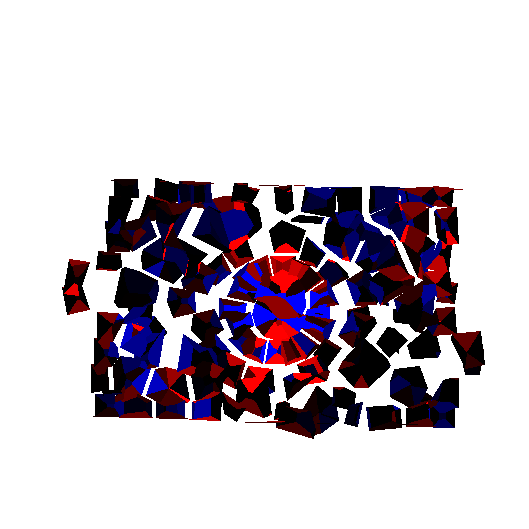
\includegraphics[width=1.0\linewidth]{Files/Small_ASR/Free_IS2/DEP5-STEP(100).png}
      \caption{Loading Step 80}
      \end{subfigure}%
      %*******
      \begin{subfigure}{.33\textwidth}
        \centering
        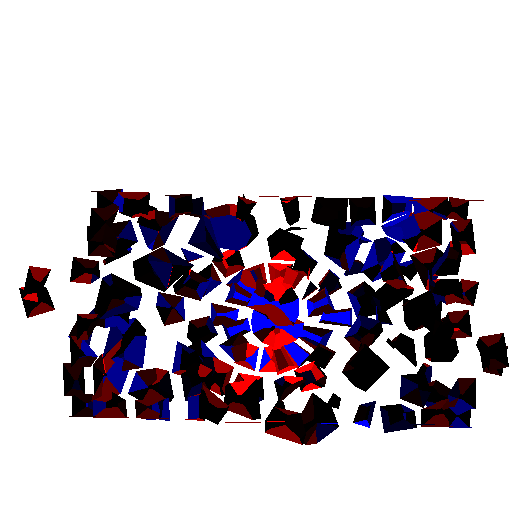
\includegraphics[width=1.0\linewidth]{Files/Small_ASR/Free_IS2/DEP5-STEP(120).png}
        \caption{Loading Step 100}
      \end{subfigure}
      %*******

  \caption{ASR Loading for 10x10x10mm model, Free Boundary Condition}
  \label{fig:ASR_Loading_s_free}
\end{figure}

From the small size model it can be confirmed the workability of uni-axial compression test on a single aggregate 10x10x10mm model. Later, uni-axial compression test on full size model(100x100x100mm) damaged by ASR expansion will be carried out.
